Las pruebas unitarias son una pieza esencial del código de calidad. Sirven para tener la certeza de que al usuario le llega siempre una versión de la aplicación que funciona como se espera. Si se desea conocer más sobre las pruebas unitarias, recomiendo conocer la historia de \citet{WHYUNT}. 

En cualquier caso, cualquier aplicación con potencial de crecimiento necesita pruebas automáticas. En el mercado hay una infinidad de herramientas que nos resuelven este problema. Aunque en el caso de React, solo hay unas pocas que estén recomendadas oficialmente por el equipo de React. Como se especifica en la documentación (\cite{RETEUT}), se recomienda utilizar Jest junto con una de las siguientes librerías: React Testing Library o Enzyme. Jest parece la opción clara, dado que es la que utiliza Facebook (creadores de React), es la que más se utiliza en el mercado y es la que más satisfacción genera, como se puede comprobar en la figura \cref{fig:stjs2019:unit-testing}.

El dilema surge entre Enzyme y React Testing Library. ¿Qué diferencia hay entre ellos? Como primera respuesta, recomiendo leer la que ha dado \citet{EVRUVRL} en Stack Overflow. Básicamente, Enzyme nos permite acceder a los métodos de nuestros componentes y React Testing Library siempre simula el componente completo. Además, Enzyme permite algo llamado Shallow Render. Esto significa dibujar únicamente el componente que se desea probar, simulando sus hijos. Enzyme es más fácil de utilizar, pero más peligroso y, a la larga, menos mantenible. El hecho de que React Testing Library nos obligue a utilizar los componentes tal y como se renderizan en un ambiente de producción implica tener más seguridad en nuestro código, tal y como explica \citet{NVSHRD} en su artículo y, posteriormente, revisa \citet{RVRT19} en 2019. La filosofía es sencilla: es mejor hacer pruebas que den la confianza de que el código funciona y no emularlo.

Por estos motivos, las pruebas unitarias van a ser mediante Jest y React Testing Library, que son las herramientas recomendadas oficialmente. Durante el transcurso de este trabajo, se valorará utilizar Enzyme haciendo comprobaciones sobre la curva de aprendizaje y la velocidad en proyectos más pequeños, pudiendo ser implementado como opción. Sin embargo, como este entorno pretende ser útil en proyectos con potencial de crecimiento, se preferirá el uso de React Testing Library por su mejor mantenibilidad.

\begin{figure}
	\centering
	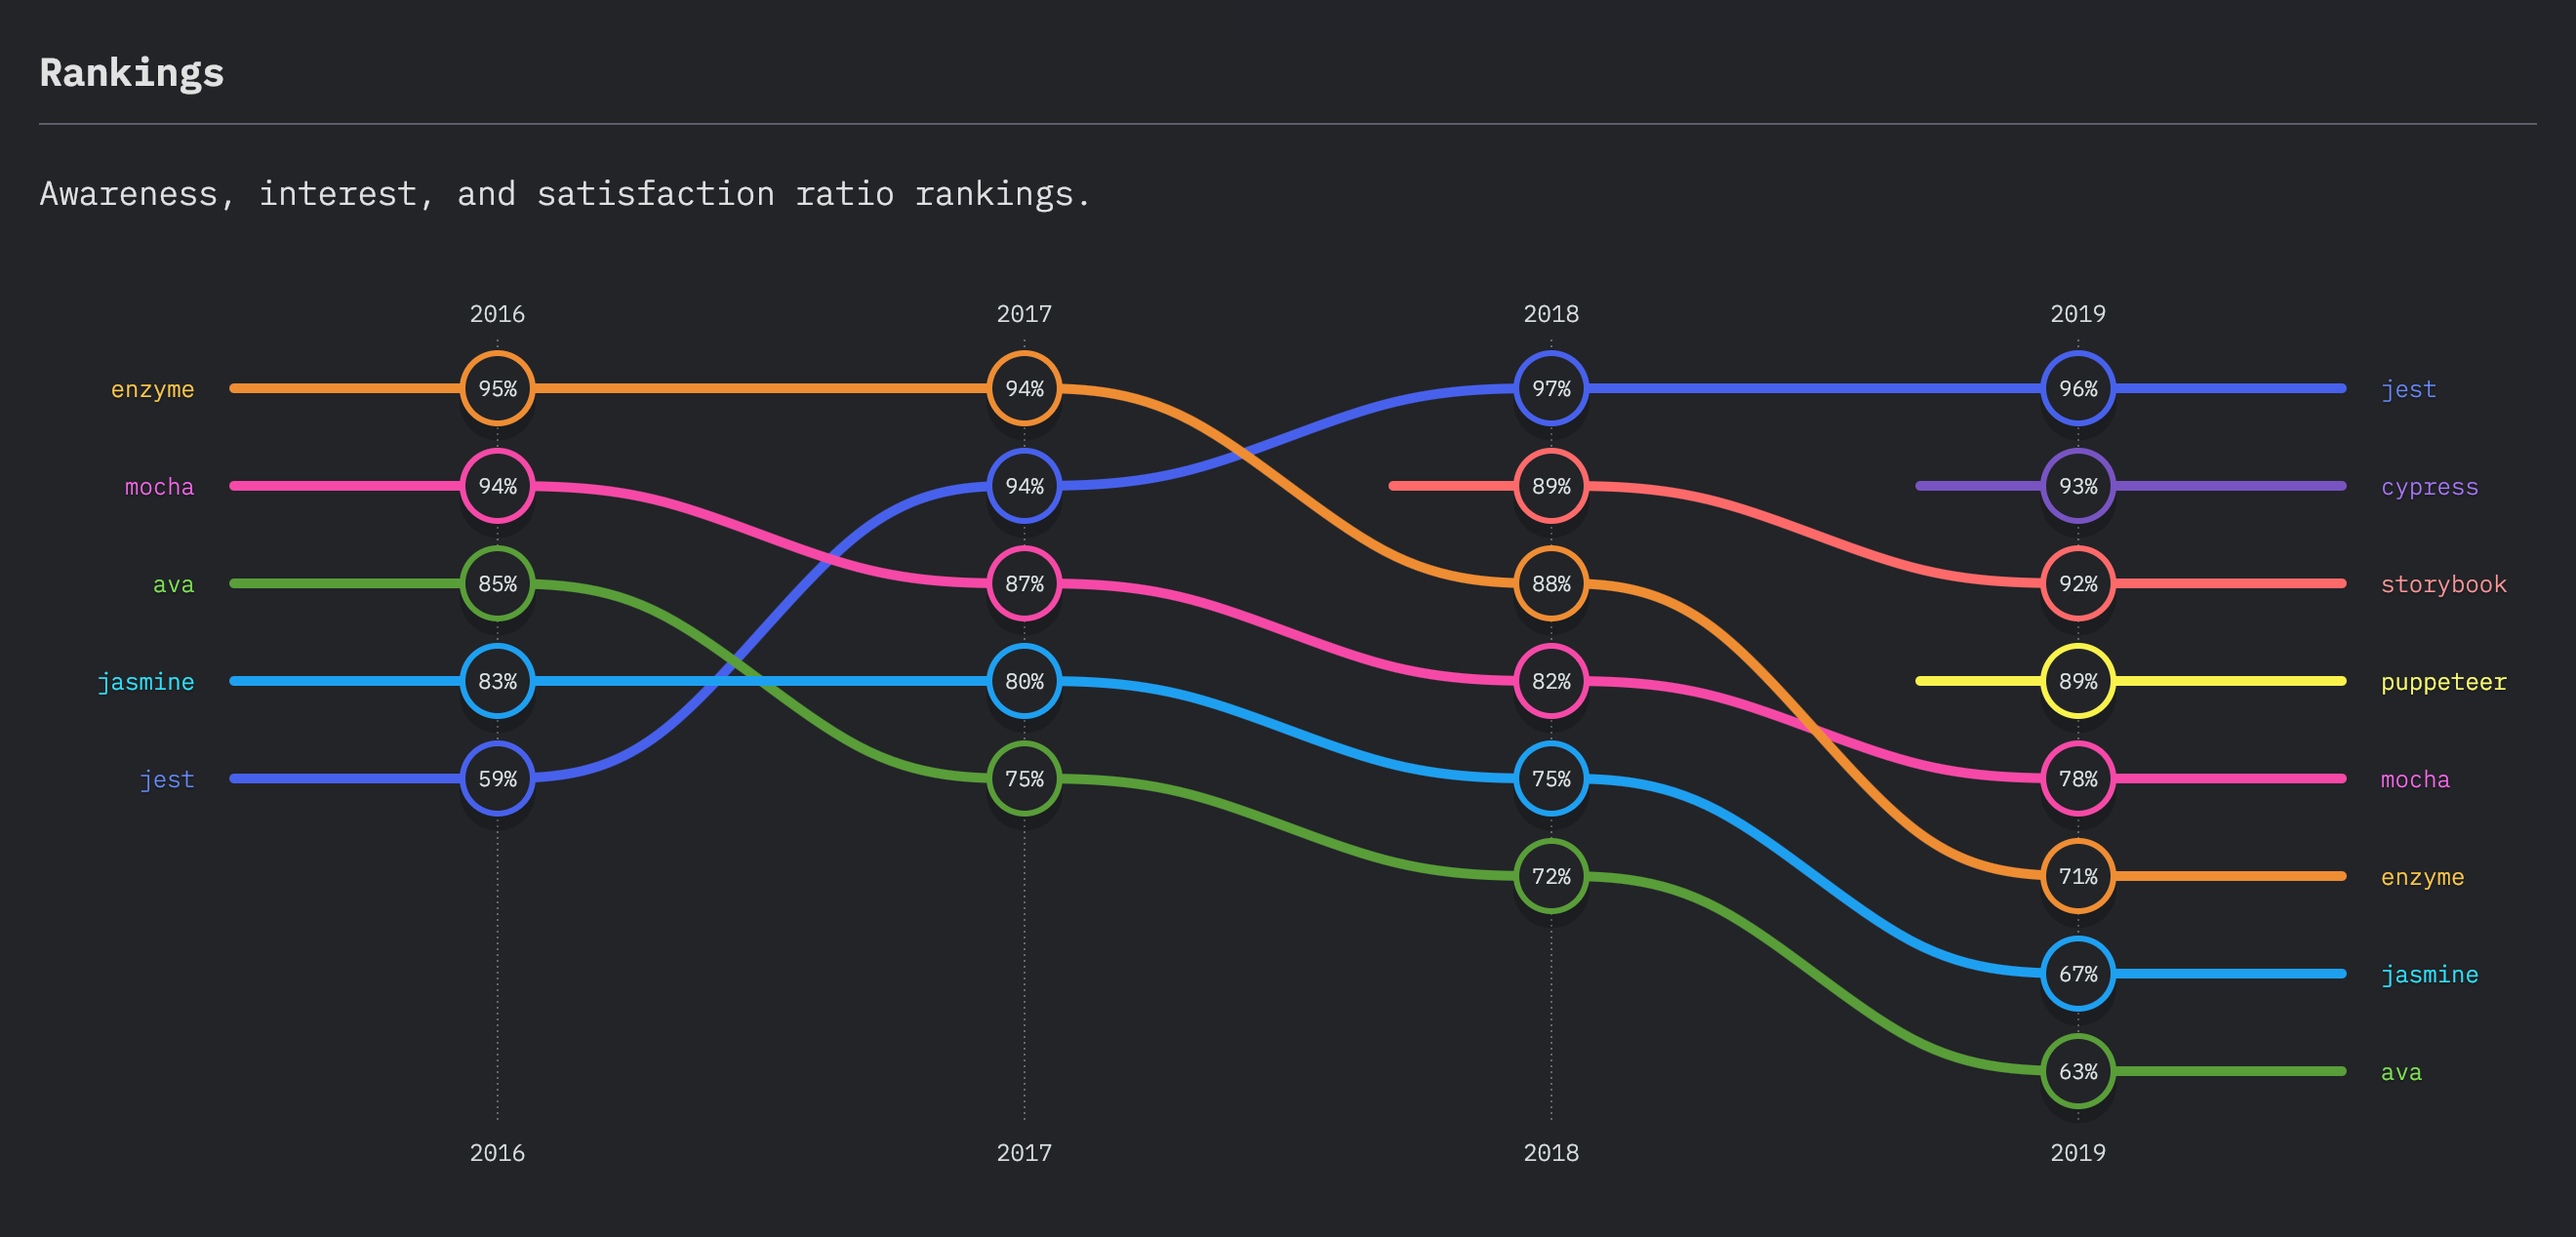
\includegraphics[width=\textwidth]{testing_experience_ranking.png}
	\caption{2019 - Opinión popular de las herramientas de pruebas unitarias}
	\label{fig:stjs2019:unit-testing}
\end{figure}